\section{Approche non-supervisée par GMM}

\textbf{Question 1: Description apprentissage du classifieur non supervisé gaussien} \\

L'apprentissage d'un classifieur non supervisé basé sur les mélanges de gaussiennes se déroule en plusieurs étapes.

\begin{enumerate}
    \item Initialisation des paramètres
    \item Expectation-Maximization (Calculer la probabilité d'appartenance à chaque composant pour chaque données et mettre à jour les paramètres du modèle en maximisant la log-vraisemblance du jeu de données)
    \item Clustering (Utiliser les responsabilités pour attribuer chaque point de données à la composante la plus probable)
\end{enumerate}




\clearpage 

\textbf{Question 2: Classifieur basé des mélanges gaussiennes} \\

\textbf{Visualisation des descripteurs d’apprentissage et de leur classe} \\

\begin{figure}[!h]
    \begin{minipage}{.48\linewidth}
        \begin{center}
            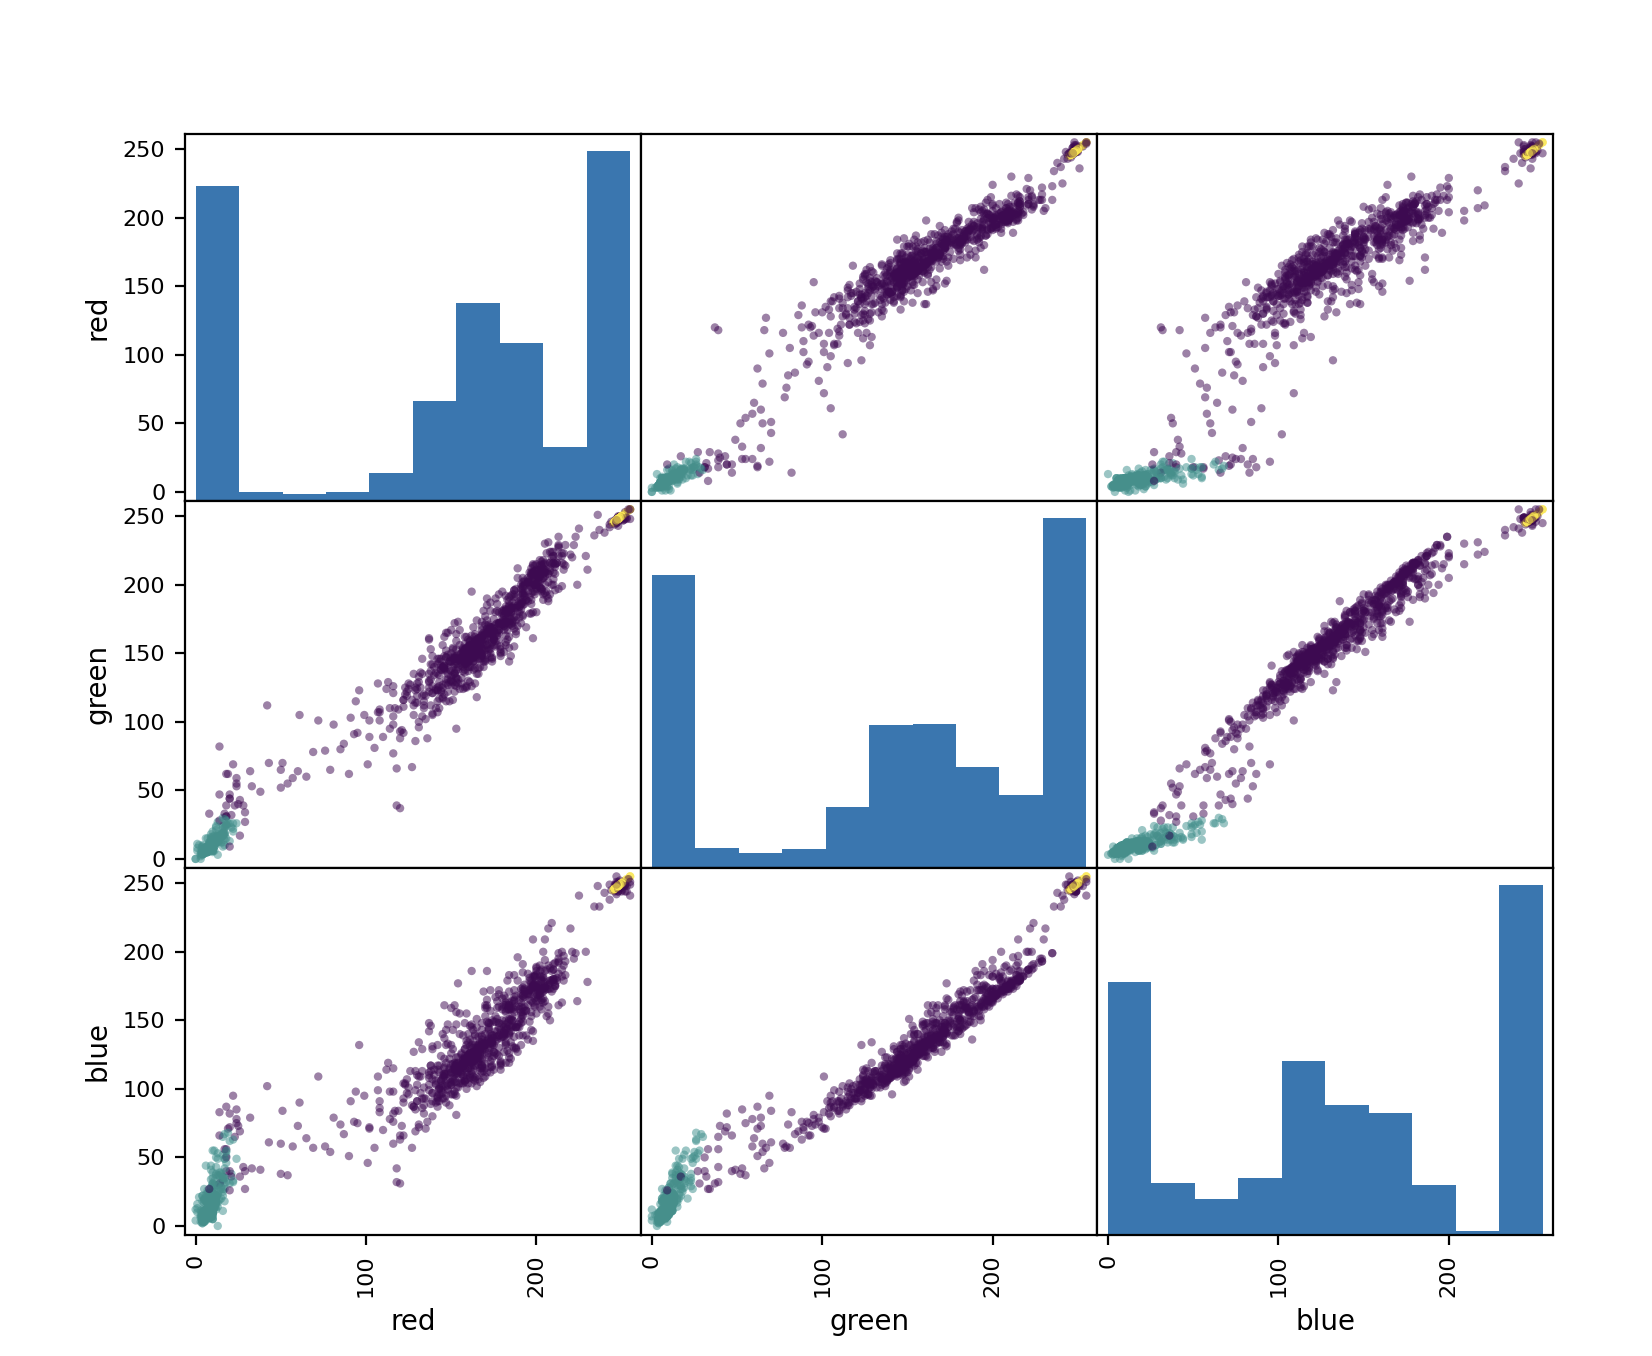
\includegraphics[width=0.75\textwidth]{./img/7.2.1.png}
                \caption{\label{fig:6.4.1}Image 2D Gauss}  
            \end{center}
    \end{minipage}\hfill
    \begin{minipage}{.48\linewidth}
        \begin{center}
            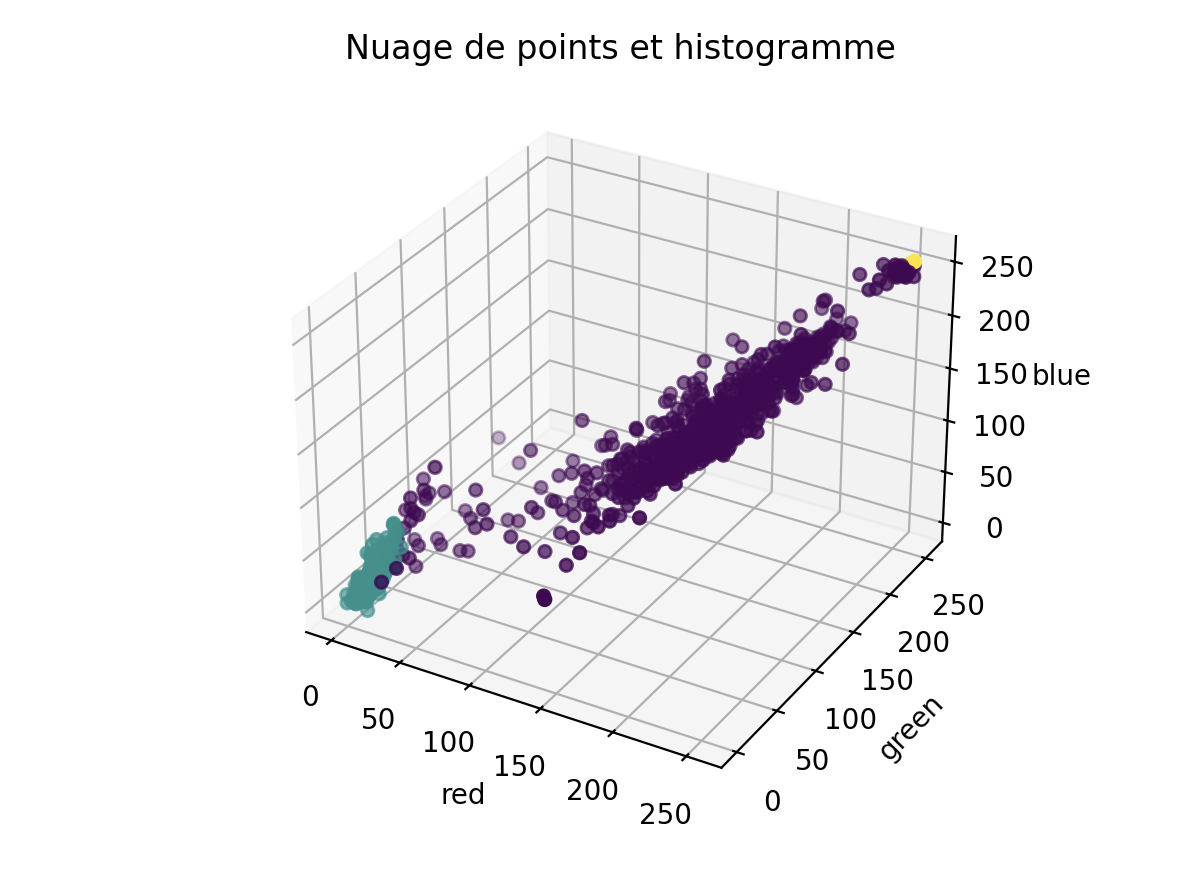
\includegraphics[width=0.75\textwidth]{./img/7.2.2.png}
            \caption{\label{fig:6.4.2}Image 3D Gauss}  
        \end{center}
    \end{minipage}
\end{figure}




\textbf{Visualisation de la classification des deux images} \\

Le code est le même, on a simplement modifié la méthode utilisée dans unsupervisedTraining.


\begin{figure}[!h]
    \begin{minipage}{.48\linewidth}
        \begin{center}
            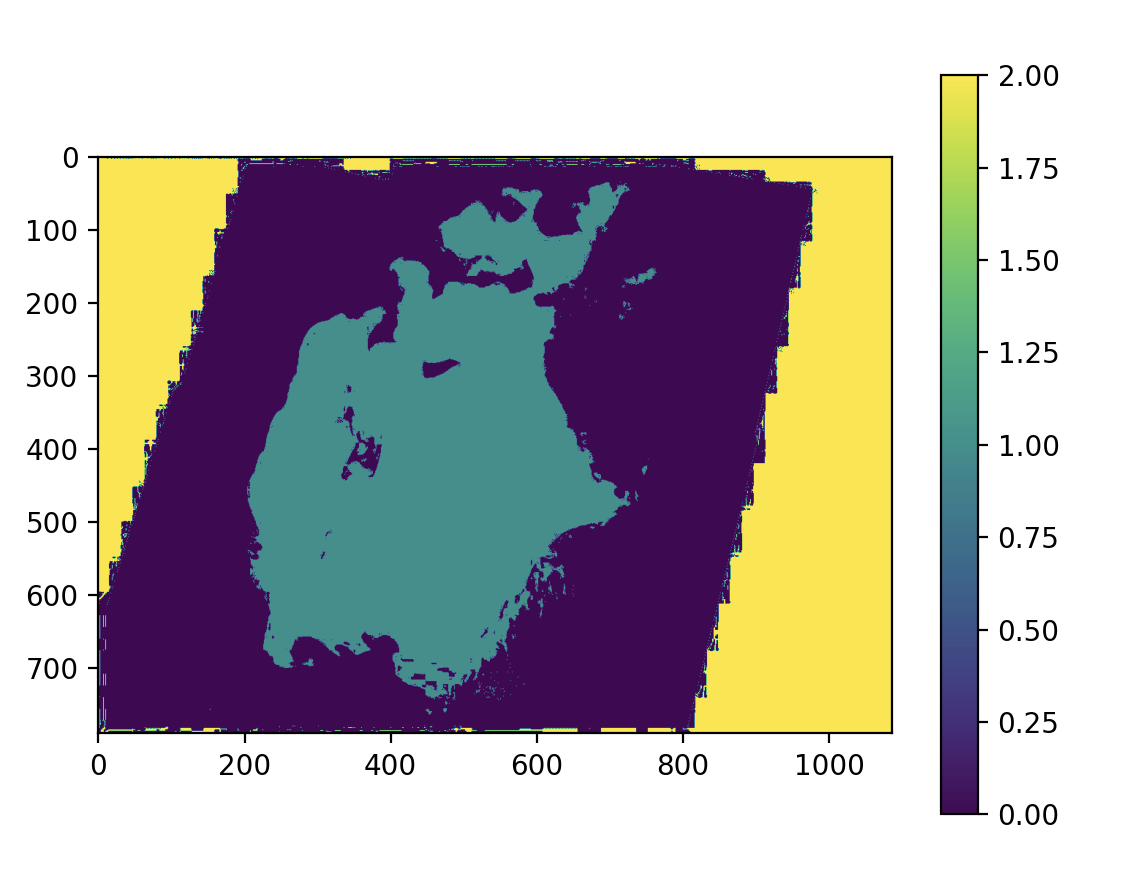
\includegraphics[width=0.75\textwidth]{./img/7.2.3.png}
                \caption{\label{fig:6.4.1}Image 1973 Predicted Labels Gauss}  
            \end{center}
    \end{minipage}\hfill
    \begin{minipage}{.48\linewidth}
        \begin{center}
            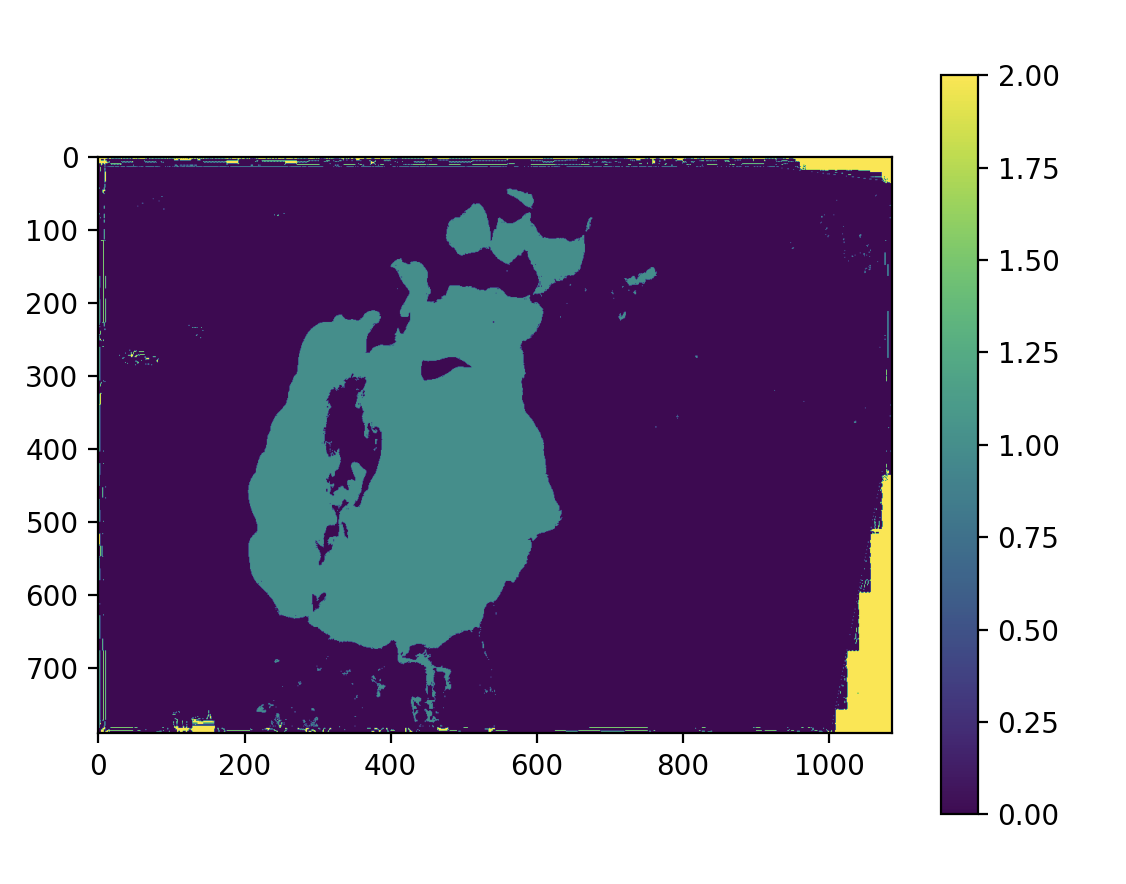
\includegraphics[width=0.75\textwidth]{./img/7.2.4.png}
            \caption{\label{fig:6.4.2}Image 1987 Predicted Labels Gauss}  
        \end{center}
    \end{minipage}
\end{figure}



















